\section{Double Beta Processes}\label{sec:doublebeta}

\subsection{Neutrinoless Double Beta Decay of \texorpdfstring{$^{136}$Xe}{Xenon-136}} \label{sec:0nubb}

Among the main intellectual challenges facing the nuclear and particle physics communities today are the neutrino-mass generation mechanism, the absolute neutrino-mass scale, and the neutrino-mass spectrum. One of the best ways to address these fundamental questions is to search for neutrinoless double beta decay ($0\nu\beta\beta$)~\cite{Avignone:2007fu, Dolinski:2019nrj}. The observation of this rare nuclear decay process, forbidden in the Standard Model, would imply that the lepton number is violated by two units and confirm the Majorana nature of the neutrinos. Double beta decay can occur in the two xenon isotopes $^{134}$Xe~\cite{LZ:2021rff} and $^{136}$Xe, with the latter offering a larger sensitivity to the $0\nu\beta\beta$ half-life ($T^{0\nu}_{1/2}$). The best experimental constraint on the $^{136}$Xe $0\nu\beta\beta$ half-life, $T^{0\nu}_{1/2} > 1.07 \times 10^{26}\1{years}$ (90\% CL), is set by the KamLAND-Zen collaboration using $^{136}$Xe dissolved in a liquid scintillator~\cite{KamLAND-Zen:2016pfg}. The EXO-200 collaboration demonstrated that better energy resolution and background rejection can be achieved with a liquid xenon TPC~\cite{Albert:2017owj}, and the PandaX-II collaboration conducted a first search using a dual-phase natural xenon detector~\cite{Ni:2019kms}. XENON1T recently demonstrated that energy resolutions below $\sigma/\mu=1$\% at $Q_{\beta\beta}$ can be achieved in liquid xenon TPCs used for dark matter searches~\cite{XENON:2020iwh}.

\begin{figure}[!htbp]
\begin{center}
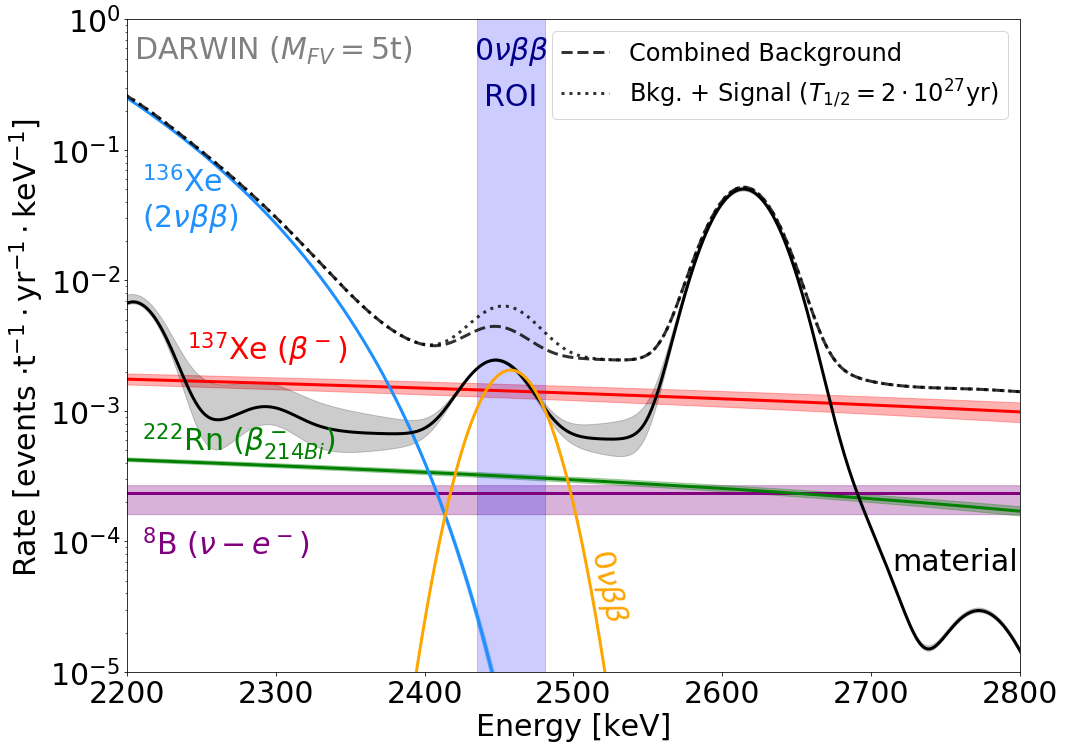
\includegraphics[width=0.99\columnwidth]{fig_0vbb_signal.png}
\caption{Predicted  background  spectrum around the $0\nu\beta\beta$ energy region of interest (ROI) for a proposed next-generation dark matter experiment. Rates are averaged over a fiducial volume (FV) containing $5000\1{kg}$ of liquid xenon with natural isotopic abundance. Bands indicate $\pm~1\sigma$ uncertainties. Figure from~\cite{Agostini:2020adk}.}\label{fig:0vbb_signal}
\end{center}
\end{figure}

A next-generation liquid xenon detector will contain multiple tonnes of the $^{136}$Xe isotope, either at the natural abundance of 8.9\%, or, as a possible upgrade, using enriched xenon. Given a TPC design optimized for WIMP searches, a detector instrumenting $\sim 40,000\1{kg}$ of non-enriched xenon can already improve the sensitivity to $0\nu\beta\beta$ decay by more than one order of magnitude over current limits, without any interference with its primary dark matter science goal. Taking advantage of the excellent self-shielding of liquid xenon, the material-induced gamma ray background can be suppressed below the total intrinsic background rate (\autoref{sec:erfiducialization}. \autoref{fig:0vbb_signal} shows the relevant sources of background with a hypothetical $0\nu\beta\beta$ signal for the innermost $5000\1{kg}$ of natural xenon in the TPC of a proposed next-generation detector~\cite{Agostini:2020adk}. The background from material-induced gamma rays will be further reduced in more massive detectors than the one simulated in \autoref{fig:0vbb_signal}.

\begin{figure}[!htbp]
\begin{center}
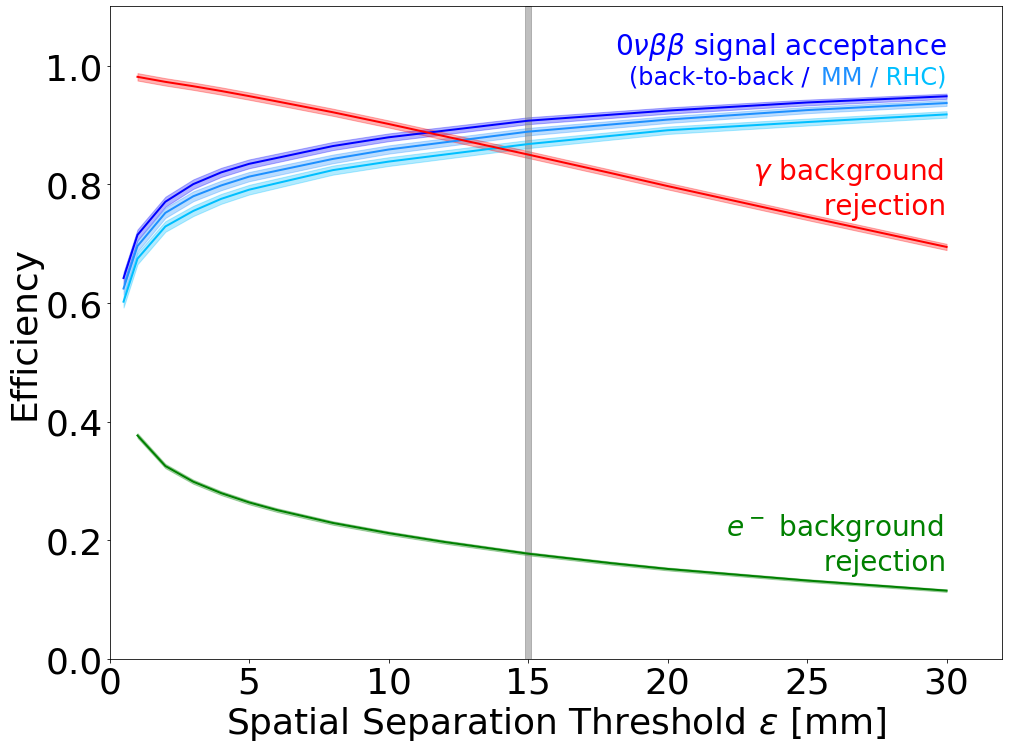
\includegraphics[width=0.99\columnwidth]{fig_0vbb_acceptance.png}
\caption{Efficiency of $0\nu\beta\beta$ signal acceptance and background rejection as a function of the minimum distance for individual reconstruction of energy depositions. The three signal lines (blue) compare different energy and angular distributions for the $0\nu\beta\beta$ signal based on a back-to-back electron emission, a mass mixing (MM) mechanism and a right-handed current (RHC) model. The background rejection efficiency is shown for $\gamma$s (red) and electrons (green) with $E=Q_{\beta\beta}=2457.8\1{keV}$. The vertical line (gray) corresponds to the value assumed here. Bands indicate $\pm~2\sigma$ uncertainties~\cite{Agostini:2020adk}.}\label{fig:0vbb_acceptance}
\end{center}
\end{figure}

\begin{figure}[!htbp]
\begin{center}
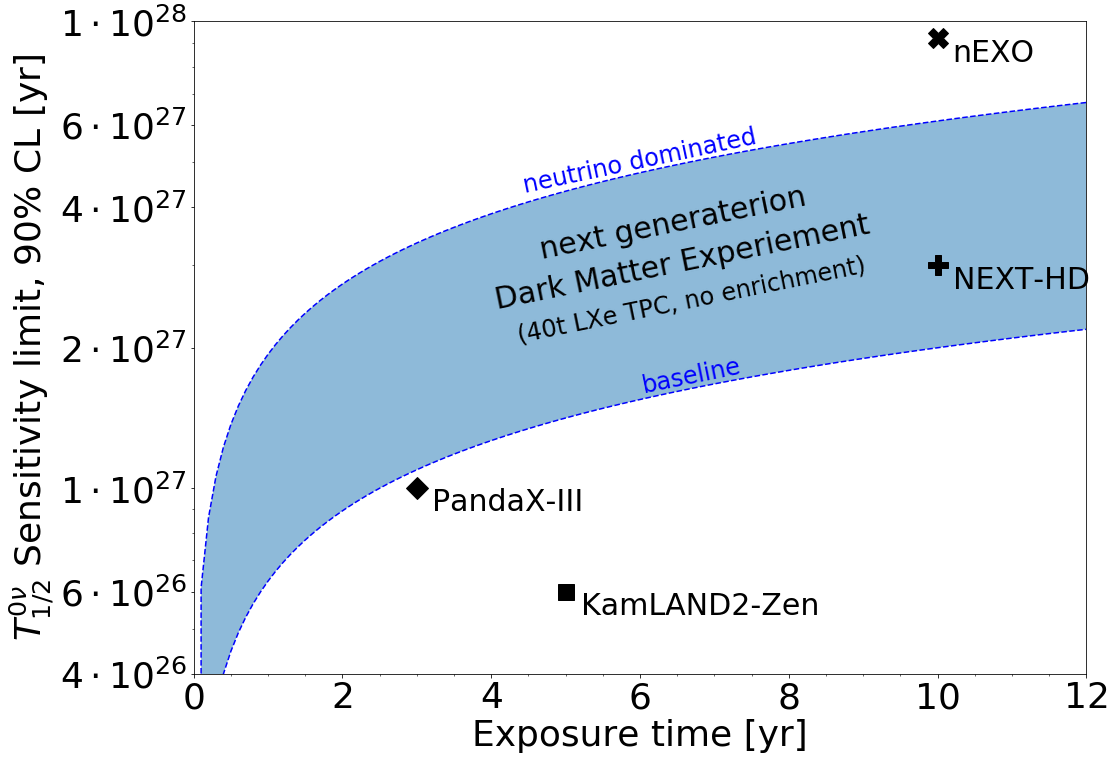
\includegraphics[width=0.99\columnwidth]{fig_0vbb_sensitivity.png}
\caption{Predicted median $T_{1/2}^{0\nu}$ sensitivity at 90\%~CL as a function of the exposure time for a next generation TPC detector containing \SI{40}{t} of liquid xenon with natural isotopic abundance. The band indicates the sensitivity range between a baseline radio purity scenario at a depth of \SI{3500}{m} water equivalent to a scenario with neutrino dominated background. Sensitivity projections for future $^{136}$Xe $0\nu\beta\beta$ experiments~\cite{Agostini:2020adk, Gomez_NEXT:2019, Chen:2016qcd, Albert:2017hjq, Barabash:2015eza} are shown for comparison.}\label{fig:0vbb_sensitivity}
\end{center}
\end{figure}

Selecting ultra-low background materials for construction can further reduce the material contribution as well as the background rate from $^{222}$Rn, which emanates from material surfaces into the target volume. A sufficiently deep laboratory suppresses cosmogenic background sources, such as the in-situ activation of $^{136}$Xe by muon-induced neutrons (producing $^{137}$Xe)~\cite{Cebrian:2020bwn,Rogers:2020npx}, down to the limit set by electron scattering of solar $^{8}$B neutrinos. Optimizing the detector design for an improved spatial resolution would allow to further exploit background rejection, based on the different topology of background and signal events caused by Bremsstrahlung radiation, as shown in \autoref{fig:0vbb_acceptance}. Combining these measures, the experimental sensitivity can be further enhanced to make a next-generation dark matter detector competitive to dedicated next-generation, tonne-scale $0\nu\beta\beta$ experiments, as shown in \autoref{fig:0vbb_sensitivity}. Isotopic enrichment in $^{136}$Xe would further improve this sensitivity, as it linearly increases the signal, although this also increases the background rate from the two-neutrino double beta decay ($2\nu\beta\beta$) of $^{136}$Xe and $\beta$-decay of $^{137}$Xe.

Besides the search for $0\nu\beta\beta$ decay, precision measurements of the $2\nu\beta\beta$ decay can reduce the experimental uncertainty on the $2\nu\beta\beta$ nuclear matrix and constrain the underlying nuclear theories~\cite{Saakyan:2013yna}.  Recent research shows that precise $2\nu\beta\beta$ spectrum shape measurement can provide insights towards reliable $0\nu\beta\beta$ nuclear matrix element calculations~\cite{KamLAND-Zen:2019imh}. In addition, precision measurements of $2\nu\beta\beta$ decay can also be used to probe New Physics. For example, right-handed lepton currents affect the angular and energy distributions of the decay \cite{Deppisch:2020mxv}, MeV-scale sterile neutrinos can be searched for through kinks in the $2\nu\beta\beta$ spectrum \cite{Bolton:2020ncv, Agostini:2020cpz}, and neutrino self-interactions can leave an imprint on the spectrum as well \cite{Deppisch:2020sqh}. Because lepton number is not necessarily violated in $2\nu\beta\beta$ decay, this is independent of the neutrino nature and can be used to constrain or pinpoint properties of both Majorana and Dirac neutrinos.

\subsection{Double Electron Capture on \texorpdfstring{$^{124}$Xe}{Xenon-124}}\label{sec:dec}

Similar to double beta decay, double electron capture is a second order Weak Interaction process~\cite{Winter:1955zz} with extremely long half-lives. Two electrons are captured from the atomic shell and two protons are converted into neutrons. In the Standard Model decay, two neutrinos carrying virtually the total Q-value are emitted and leave the active volume undetected ($2\nu$ECEC). The measurable signal is constituted by the atomic de-excitation cascade of X-rays and Auger electrons that occurs when the vacancies of the captured electrons are refilled. In a liquid xenon detector, this cascade is measured as a single resolvable signal at $64.3\1{keV}$ for the double K-capture~\cite{Nesterenko:2012xp} as the most likely case~\cite{Doi:1991xf}. The half-life of this decay is of great interest with regard to nuclear matrix element calculations, as it provides a benchmark point from the proton-rich side of the nuclide chart~\cite{Suhonen:2013rca,Pirinen:2015sma,Perez:2018cly}. A precise measurement would help to narrow down uncertainties, which in turn have implications on the neutrino mass scale derived from $0\nu\beta\beta$. 

Following hints in XMASS~\cite{Abe:2018gyq}, the half-life of the $^{124}$Xe double K-capture has recently been measured by XENON1T~\cite{XENON:2019dti}. At $T_{1/2}^{2\nu\text{KK}} = (1.8 \pm 0.5_\text{stat} \pm 0.1_\text{sys}) \times 10^{22}\1{years}$, it agrees with recent theoretical predictions. Assuming a natural isotopic abundance similar to XENON1T, a next-generation experiment would record on the order of 10,000 events in its full exposure. This will allow a precision measurement of the double K-capture half-life to the percent level. Additionally, an observation of the KL-capture and LL-capture would be within reach~\cite{Doi:1991xf}. Their measurement would help to decouple the nuclear matrix element from phase-space factors.

Beyond the Standard Model, the double electron capture on $^{124}$Xe without neutrino emission ($0\nu$ECEC) can complement $0\nu\beta\beta$ in addressing fundamental questions about the mass and nature of the neutrino~\cite{Bernabeu:1983yb,Sujkowski:2003mb}. $^{124}$Xe could allow a resonant enhancement of this channel, which would be needed to provide accessible half-lives~\cite{Kotila:2014zya}. In this case, the decay populates an excited state of the $^{124}$Te daughter nucleus. A suitable daughter state exists, but current measurements of the Q-value indicate only an approximate match of the $^{124}$Te level, two-hole energy, and Q-value that would only provide a minor enhancement~\cite{Nesterenko:2012xp}. If this decay is realized, the experimental signature contains multiple $\gamma$-rays emitted in a cascade, so coincidence techniques could increase experimental sensitivity \cite{Wittweg:2020fak}.

\subsection{Other Double-Beta Processes}

The $^{124}$Xe $Q$-value of 2857~keV also allows second-order decays involving positrons. Examples are the as-yet unobserved Standard Model $2\nu$EC$\beta^+$ and $2\nu\beta^+\beta^+$ decays, as well as the hypothetical $0\nu$EC$\beta^+$ and $0\nu\beta^+\beta^+$ decays. The decay $2\nu$EC$\beta^+$ is predicted to have a half-live one order of magnitude above that of $2\nu$ECEC. Exploiting the coincidence signature of the positron annihilation and the atomic de-excitation cascade, this decay could already be within reach of LZ and XENONnT~\cite{Barros:2014exa, Wittweg:2020fak} and be a sure signal in the next-generation detector. The $2\nu\beta^+\beta^+$ decay exhibits a unique signature with five point-like ionization clusters, located in the same plane with the central vertex~\cite{Bolozdynya:1997pdbd}.

On the neutrinoless side, $0\nu$EC$\beta^+$ would be favoured in the absence of resonance enhancement for $0\nu$ECEC. Here, the current lower limits on the half-lives are on the order of~\SIrange{e25}{e27}{years}~\cite{Barea:2013wga, Kim:1982vi, Doi:1992dm, Hirsch:1994es, Suhonen:2003gx, Rath:2009dr, Wittweg:2020fak}. These would be accessible to a large extent in a next-generation liquid xenon experiment when exploiting the coincidence signature of the atomic relaxation, the mono-energetic positron, and the two subsequent back-to-back $\gamma$-rays. Moreover, limits on half-lives of neutrinoless second-order weak decays in $^{124}$Xe could complement $0\nu\beta\beta$ searches in $^{136}$Xe and help to identify the decay mechanism~\cite{Hirsch:1994es, Wittweg:2020fak}. These channels provide an exciting avenue for the next-generation detector discussed here to complement ongoing searches for double-weak processes.




